\documentclass[conference]{IEEEtran}
\IEEEoverridecommandlockouts

\usepackage{cite}
\usepackage{amsmath,amssymb,amsfonts}
\usepackage{algorithmic}
\usepackage{graphicx}
\usepackage{textcomp}
\usepackage{xcolor}
\usepackage{booktabs}
\usepackage{multirow}
\usepackage{url}
\def\BibTeX{{\rm B\kern-.05em{\sc i\kern-.025em b}\kern-.08em
    T\kern-.1667em\lower.7ex\hbox{E}\kern-.125emX}}

\begin{document}

\title{Frozen-Expert MoE for\\Code-Mixed Language Modeling for\\Indian Social Media}

\author{
\IEEEauthorblockN{Priyanshu Narayan, Samarth Agrawal, Satyasheel Singh, Vaishnav Vaijnath Pasarge}
\IEEEauthorblockA{\textit{Department of Computer Science}\\
\textit{CS F425 - Deep Learning}\\
BITS Pilani \\
\{f20230283; f20230761; f20230261; f20230631\}@pilani.bits-pilani.ac.in}}

\maketitle

\begin{abstract}
Hindi-English code-mixing is pervasive on Indian social media, where speakers switch freely between languages mid-sentence. Standard NLP models, trained on monolingual data, struggle here because no single model handles both Hindi morphology and English semantics well. The obvious fix-fine-tuning a multilingual model end-to-end-is expensive, risks overwriting useful pre-trained representations, and forces one set of weights to handle two linguistically distinct token types at once.

We propose \textbf{Frozen-Expert Mixture of Experts (FE-MoE)}, which takes a different route: keep two complementary pre-trained models-HingBERT \cite{nayak2022hingbert} and RoBERTa-base \cite{liu2019roberta}-entirely frozen, and train only a small router ($\sim$200K parameters) that learns, per token, how much weight to place on each expert. The router must compensate for representation mismatch between two independently trained models, operate across two different tokenisation schemes, and learn to route by language with no direct language supervision.

We evaluate on Language Identification (LID) and Part-of-Speech (POS) tagging using COMI-LINGUA \cite{sheth2024comilingua}. Our best configuration reaches \textbf{88.98\% weighted F1 on LID}, within 0.67 points of a fully fine-tuned HingBERT (89.65\%), while training only \textbf{0.24\% as many parameters}. Analysis of the learned routing weights shows the router picks up language-specific patterns without ever seeing a language label.
\end{abstract}

\begin{IEEEkeywords}
code-mixing, mixture of experts, Hinglish, language identification, POS tagging, frozen experts, soft routing, parameter-efficient
\end{IEEEkeywords}

% ─────────────────────────────────────────────
\section{Introduction}
% ─────────────────────────────────────────────

Code mixing, which is switching between languages within a single sentence is simply how a large share of Indian social media users write. A post like \textit{``Yaar yeh movie was actually amazing, bilkul waste of time nahi tha''} is entirely normal, yet it breaks both Hindi and English NLP pipelines. You need both languages at once, and most models are not built for that \cite{nayak2022hingbert,aguilar2020lince}.

The problem is more tricky than it looks. Annotated code-mixed data is scarce; most corpora are Twitter scrapes with inconsistent romanisation. Spelling variation is extreme -\textit{``nahi''}, \textit{``nahin''}, \textit{``nhi''} are all the same word- which trips up vocabulary-based methods. And any model has to simultaneously track Hindi morphology and English syntax within the same sentence.

\textbf{Why not just fine-tune?} Fine-tuning a pre-trained model like HingBERT is the natural first step, and it works. But it updates all $\sim$85M parameters, which is slow and memory intensive. It also risks erasing the very representations that made HingBERT good at Hinglish in the first place. Perhaps more fundamentally, it collapses everything into one set of weights even though Hindi tokens and English tokens arguably want to be handled by different specialised representations.

\textbf{Our approach.} Instead, we freeze two complementary pre-trained models and learn only a small router that blends their outputs for each token. This is genuinely harder than fine-tuning in two ways: the router must align the hidden-state geometry of two models trained completely independently, and it must figure out which language a token belongs to purely from downstream task loss -no language labels ever reach the router.

We focus on two sequence labelling tasks: Language Identification (LID), which labels each token as Hindi, English, or Other, and Part-of-Speech (POS) tagging. LID is a prerequisite for basically any downstream code-mixed application. POS tests whether the model has picked up syntactic structure across language boundaries. Together they give a good sense of how well the model actually understands the text.

Our main contributions are:
\begin{enumerate}
  \item A frozen dual-expert MoE framework with three router designs: MLP, BiGRU, and CNN.
  \item Ablations over temperature ($\tau$), routing granularity, and router input -13 configurations in total.
  \item Evidence that 200K parameters can match 85M-parameter fine-tuning on LID.
  \item Interpretability results showing the router learns language-aware routing with no explicit supervision.
\end{enumerate}

% ─────────────────────────────────────────────
\section{Related Work}
% ─────────────────────────────────────────────

\subsection{Code-Mixed NLP}

HingBERT \cite{nayak2022hingbert} is a BERT-base model pre-trained on 52.93 million Hindi-English tweets, making it a natural choice for Hinglish tasks where multilingual BERT falls short. We use it as our Hindi-specialist expert. The LinCE benchmark \cite{aguilar2020lince} brought some standardisation to code-switching evaluation, motivating our choice of LID and POS as the core tasks. Our experiments use COMI-LINGUA \cite{sheth2024comilingua}, a recent expert-annotated dataset covering Hindi-English LID, POS, and NER with strong inter-annotator agreement ($\kappa \geq 0.81$)-one of the more carefully constructed resources in this space.

\subsection{Mixture of Experts}

Shazeer et al.\ \cite{shazeer2017moe} showed that routing tokens to sparse expert sub-networks could scale model capacity without proportional compute increases. Puigcerver et al.\ \cite{puigcerver2024softmoe} replaced discrete routing with a fully differentiable soft assignment-the direct inspiration for our approach. MoEBERT \cite{zuo2022moebert} restructures a pre-trained BERT into an MoE via importance-guided distillation; unlike that work, we never touch the expert weights at all. MoE-LPR \cite{zhou2024moelpr} is probably the closest conceptually to what we do-it uses language-prior routing to extend an LLM to new languages-but the setting is monolingual expansion rather than mixing two languages in the same sentence. On the speech side, LR-MoE \cite{wang2023lrmoe} does frame-level language routing for code-switched ASR; our results suggest an analogous signal can emerge in text without explicit LID labels.

% ─────────────────────────────────────────────
\section{Dataset and Task Formulation}
% ─────────────────────────────────────────────

\subsection{COMI-LINGUA}

COMI-LINGUA \cite{sheth2024comilingua} is an expert-annotated Hindi-English code-mixed corpus drawn from social media, covering LID, POS, and NER. We keep only romanised sentences (Devanagari-script sentences are filtered out) and follow the provided train/dev/test split, holding out 10\% of training data for validation.

\subsection{Tasks}

\textbf{Language Identification (LID)} tags each token as \texttt{hi} (Hindi), \texttt{en} (English), or \texttt{ot} (Other). Getting this right is a prerequisite for everything downstream-you cannot do sentiment analysis or translation on code-mixed text reliably without it. We report weighted F1.

\textbf{Part-of-Speech Tagging (POS)} assigns one of 14 universal POS labels per token. In code-mixed text this is genuinely tricky: a Hindi verb might sit inside an otherwise English clause, and its syntactic role depends on context from both languages. We report token accuracy.

\textbf{NER} was attempted but dropped from the main evaluation because the COMI-LINGUA split we worked with did not include labelled NER training data.

% ─────────────────────────────────────────────
\section{Methodology}
% ─────────────────────────────────────────────

\subsection{Why Frozen Experts Are Hard to Route}

It is worth being explicit about why freezing both experts makes this harder than fine-tuning. In standard fine-tuning, gradients flow everywhere and the model can reshape its internal geometry to suit the task. Here, the router receives two fixed vectors-$\mathbf{h}^{\text{hing}}_i$ and $\mathbf{h}^{\text{rob}}_i$-from models that were trained completely separately and have no reason to agree on how to represent anything:

\begin{itemize}
  \item \textbf{Tokenisation mismatch}: HingBERT uses WordPiece; RoBERTa uses BPE with prepended spaces. The same word often splits differently under each tokeniser. We average sub-token hidden states to get a single word-level vector under each model, but those vectors live in spaces that were never jointly optimised.
  \item \textbf{Geometry mismatch}: The two 768-dimensional hidden spaces have different principal directions of variation. The router, operating on their concatenation, must implicitly work out a cross-space alignment before it can make sensible routing decisions.
  \item \textbf{Implicit language supervision}: Language labels never reach the router during training-only the downstream task loss does. The router has to recover which language a token belongs to purely from the geometry of frozen hidden states.
\end{itemize}

\subsection{Model Architecture}

Each word $w_i$ is tokenised separately by HingBERT's tokeniser and RoBERTa's tokeniser. Sub-token states are averaged to produce word-level vectors $\mathbf{h}^{\text{hing}}_i, \mathbf{h}^{\text{rob}}_i \in \mathbb{R}^{768}$. Both experts remain frozen throughout. A learned router produces a scalar $\alpha_i \in (0,1)$ for each token, and the blended representation is passed to a linear task head:

\begin{equation}
    \hat{\mathbf{h}}_i = \alpha_i \cdot \mathbf{h}^{\text{hing}}_i + (1 - \alpha_i) \cdot \mathbf{h}^{\text{rob}}_i
\end{equation}

\subsection{Router Architectures}

\textbf{RouterMLP} (R1--R7): Two linear layers project the concatenated states $[\mathbf{h}^{\text{hing}}_i; \mathbf{h}^{\text{rob}}_i] \in \mathbb{R}^{1536}$ to a scalar, passed through a temperature-scaled sigmoid:
\begin{equation}
    \alpha_i = \sigma\!\left(\frac{W_2\,\text{GELU}(W_1\,[\mathbf{h}^{\text{hing}}_i; \mathbf{h}^{\text{rob}}_i])}{\tau}\right)
\end{equation}
$\tau$ controls how sharp the routing is: low $\tau$ drives $\alpha$ toward 0 or 1; high $\tau$ averages the experts uniformly.

\textbf{RouterGRU} (R8): A Bidirectional GRU (hidden size 128) processes the full token sequence before projecting each step to $\alpha_i$, giving the router access to surrounding context.

\textbf{RouterCNN} (R9): A 1D convolution (kernel $k{=}5$, 128 channels) captures a 5-token window, at lower cost than the GRU.

\subsection{Routing Modes}

Two additional variants test the limits of the routing design:
\begin{itemize}
  \item \textbf{Hard routing} (R7): A straight-through estimator \cite{bengio2013ste} forces binary expert selection in the forward pass while keeping the gradient path soft.
  \item \textbf{Sentence-level routing} (R6): A single $\alpha$ is computed from the CLS tokens of both experts and broadcast to every position, testing whether per-token granularity actually matters.
\end{itemize}

% ─────────────────────────────────────────────
\section{Experimental Setup}
% ─────────────────────────────────────────────

\subsection{Baselines}

\begin{itemize}
  \item \textbf{B1}: HingBERT fully fine-tuned ($\sim$85M trainable parameters). Upper bound.
  \item \textbf{B2}: HingBERT frozen + linear head only.
  \item \textbf{B3}: RoBERTa frozen + linear head only.
  \item \textbf{B4}: Fixed 50/50 blend of both frozen experts, no learned router.
\end{itemize}

\subsection{Training Details}

All router models are trained with AdamW ($\text{lr}{=}2{\times}10^{-4}$), batch size 32, max sequence length 128, and early stopping with patience 3 (max 20 epochs). All numbers are mean $\pm$ std over two seeds \{42, 123\}, giving 26 trained models across 13 configurations.

% ─────────────────────────────────────────────
\section{Results}
% ─────────────────────────────────────────────

\subsection{Main Results}

Table~\ref{tab:main} summarises the results. The best configuration, \textbf{R2} (MLP, $\tau{=}0.1$), reaches \textbf{88.98\% weighted F1 on LID}-0.67 points below fully fine-tuned HingBERT (89.65\%)-while training only $\sim$200K parameters versus $\sim$85M, a 425$\times$ reduction. That gap is small enough to be practically irrelevant in most settings, especially given how much cheaper the router is to train.

The gap to the frozen single-expert baselines is large: B2 scores 80.55\%, B3 scores 81.48\%, and the fixed 50/50 blend (B4) hits only 80.41\%. Simply averaging the two experts does nothing; the routing has to be learned.

\begin{table}[t]
\centering
\caption{Main results (mean $\pm$ std over two seeds). LID: weighted F1; POS: token accuracy. Overall best values and best router values are bolded.}
\label{tab:main}
\setlength{\tabcolsep}{4pt}
\begin{tabular}{llcc}
\toprule
\textbf{ID} & \textbf{Description} & \textbf{LID (\%)} & \textbf{POS (\%)} \\
\midrule
B1 & HingBERT fine-tuned       & \textbf{89.65} $\pm$ 0.23 & \textbf{91.09} $\pm$ 0.11 \\
B2 & HingBERT frozen           & 80.55 $\pm$ 0.06          & 65.23 $\pm$ 0.25 \\
B3 & RoBERTa frozen            & 81.48 $\pm$ 0.01          & 63.18 $\pm$ 0.31 \\
B4 & Fixed 50/50 blend         & 80.41 $\pm$ 0.31          & 61.10 $\pm$ 0.12 \\
\midrule
R1 & MoE MLP $\tau$=1.0        & 84.37 $\pm$ 3.21          & \textbf{67.76} $\pm$ 1.50 \\
R2 & MoE MLP $\tau$=0.1        & \textbf{88.98} $\pm$ 0.65 & 66.99 $\pm$ 1.54 \\
R3 & MoE MLP $\tau$=0.3        & 88.86 $\pm$ 0.29          & 66.99 $\pm$ 1.25 \\
R4 & MoE MLP $\tau$=0.5        & 88.43 $\pm$ 0.11          & 66.91 $\pm$ 0.97 \\
R5 & MoE MLP $\tau$=2.0        & 84.40 $\pm$ 3.24          & 66.79 $\pm$ 0.28 \\
R6 & MoE sentence-level        & 81.20 $\pm$ 0.04          & 66.28 $\pm$ 0.71 \\
R7 & MoE MLP hard routing      & 87.58 $\pm$ 0.10          & 65.20 $\pm$ 0.22 \\
R8 & MoE BiGRU router          & 86.61 $\pm$ 0.63          & 64.22 $\pm$ 2.17 \\
R9 & MoE CNN ($k$=5)           & 88.29 $\pm$ 0.12          & 66.78 $\pm$ 0.01 \\
\bottomrule
\end{tabular}
\end{table}

\subsection{POS Tagging}

POS is a different story. MoE models plateau around 67\% versus B1's 91.09\%, and the frozen baselines B2 (65.23\%) and B3 (63.18\%) are already poor. This tells us the problem is not routing- instead it is that the frozen representations do not carry the kind of task-specific syntactic structure POS tagging needs. The router can reweight vectors, but it cannot change what those vectors encode. Full fine-tuning can actually shift the backbone to represent verb agreement and case distinctions; a frozen router cannot.

\subsection{Temperature Ablation}

Routing sharpness matters more than expected. Lower $\tau$ consistently gives better LID and more stable training: R2 ($\tau{=}0.1$) peaks at 88.98\% with a standard deviation of $\pm$0.65\%. At higher temperatures (R1 and R5, $\tau{=}1.0$ and $\tau{=}2.0$), performance drops to around 84\% and variance explodes to $\pm$3.2\%, with the two seeds sometimes differing by over 6 points. Near-uniform blending seems to make optimisation fragile.

\subsection{Router Architecture Comparison}

CNN (R9, 88.29\%) comes close to the top-performing MLP (R2, 88.98\%), and that's no surprise either: code-switching in code-mix language occurs at the word level, and a 5-token window is large enough to include them. The BiGRU (R8, 86.61\%) is less successful despite its additional sequence memory. We believe that the GRU holds on to old language biases between the code switches meaning it's slow to change once locked into the Hindi language setting.

\subsection{Routing Granularity and Input Ablations}

Table~\ref{tab:ablations} shows the remaining ablations. Sentence-level routing (R6: 81.20\%) is nearly as bad as the frozen baselines which is unsurprising, since a single gate value per sentence cannot handle a mid-sentence language switch. Per-token granularity is not optional in our findings.

"Hard routing" (R7: 87.58\%) is relatively effective, but it is still less effective than soft routing, and it makes sense for tokens that lie somewhere in between languages—transliterated names, romanized borrowings, morphologically hybrid. In such cases, a combination of the two specialists may be more appropriate.

One counterintuitive finding: routing from RoBERTa-only hidden states (A3: 87.42\%) outperforms routing from HingBERT-only (A2: 86.06\%), even though HingBERT is the stronger expert for Hindi. Using both concatenated (R1) also underperforms and is much less stable. Our interpretation is that RoBERTa's representations are more consistently structured across the mixed vocabulary, making them easier to route from, even if they are weaker representations as such.

\begin{table}[t]
\centering
\caption{Ablations on LID (mean $\pm$ std). All MLP, $\tau$=1.0 unless noted.}
\label{tab:ablations}
\setlength{\tabcolsep}{4pt}
\begin{tabular}{llcc}
\toprule
\textbf{Axis} & \textbf{Config} & \textbf{LID (\%)} & \textbf{$\Delta$ vs R1} \\
\midrule
\multirow{3}{*}{Router input}
  & A3: RoBERTa only   & 87.42 $\pm$ 0.08 & $+$3.05 \\
  & A2: HingBERT only  & 86.06 $\pm$ 0.24 & $+$1.69 \\
  & R1: Both (concat)  & 84.37 $\pm$ 3.21 & - \\
\midrule
\multirow{3}{*}{Granularity}
  & R7: Hard token     & 87.58 $\pm$ 0.10 & $+$3.21 \\
  & R6: Sentence-level & 81.20 $\pm$ 0.04 & $-$3.17 \\
  & R1: Soft token     & 84.37 $\pm$ 3.21 & - \\
\bottomrule
\end{tabular}
\end{table}

% ─────────────────────────────────────────────
\section{Interpretability: What the Router Learns}
% ─────────────────────────────────────────────

\begin{figure}[t]
\centering
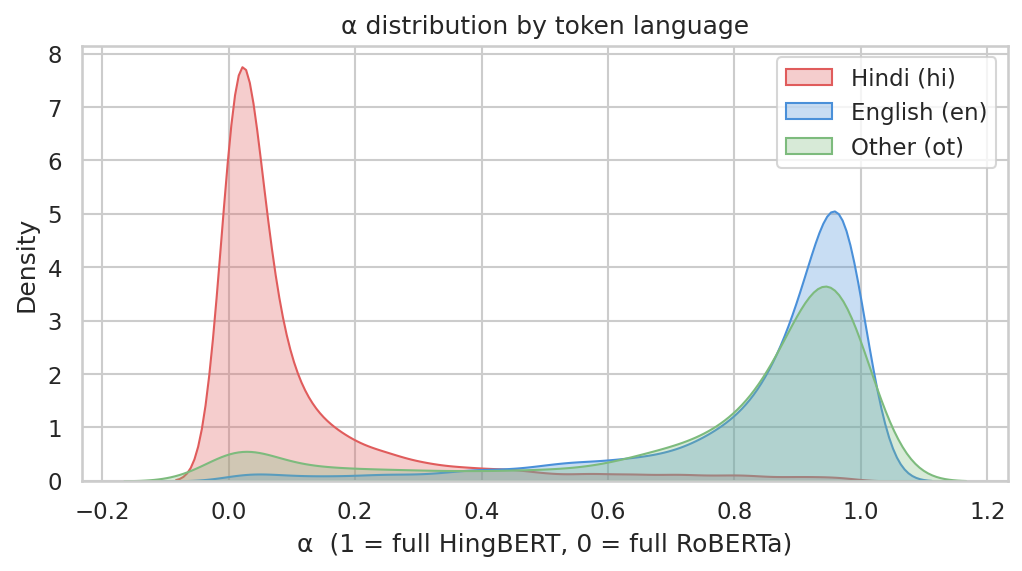
\includegraphics[width=\columnwidth]{fig_alpha_by_lang.png}
\caption{Distribution of router $\alpha$ values by gold language label (R2, seed 42, LID). Hindi tokens get higher $\alpha$ (more weight to HingBERT); English tokens get lower $\alpha$; Other falls between. No language labels were used during training.}
\label{fig:alpha_by_lang}
\end{figure}

Does the router learn anything meaningful, or does it settle on a fixed blend? Fig.~\ref{fig:alpha_by_lang} makes it clear that alpha is consistently higher for Hindi tokens compared to English tokens, with Others coming in between. This was exactly how things were expected to pan out because HingBERT should be the superior expert for Hindi tokens - and these boundaries emerge without the router ever seeing the language labels.


\begin{figure}[t]
\centering
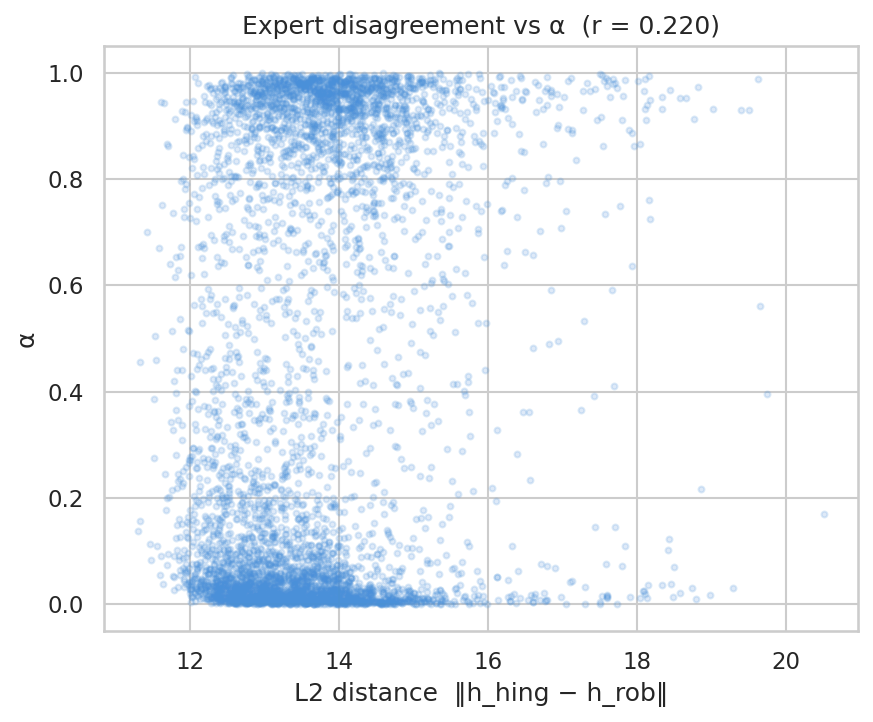
\includegraphics[width=\columnwidth]{fig_disagreement.png}
\caption{Expert hidden-state L2 disagreement vs.\ router $\alpha$ (R1, LID). Higher disagreement between the two experts produces more decisive routing-$\alpha$ closer to 0 or 1.}
\label{fig:disagreement}
\end{figure}

% ─────────────────────────────────────────────
\section{Conclusion}
% ─────────────────────────────────────────────

We introduced FE-MoE, a frozen dual-expert MoE for Hindi-English code-mixed sequence labeling. With HingBERT and RoBERTa kept frozen and only a $\sim$200K-parameter router trained, we reach 88.98\% weighted F1 on LID, whcih was within 0.67 points of full fine-tuning while using 425$\times$ fewer trainable parameters.

Across the 13 configurations we tested: low temperature ($\tau{=}0.1$) gives the best and most stable results, amd CNN routing nearly matches MLP at lower cost; sentence-level routing collapses to near-baseline performance, implying that code-mixing requires per-token decisions, and the router learns to track language identity purely from task-level feedback, with no explicit supervision.

POS tagging is the clear weak point, and it is worth being honest about why: frozen representations simply do not encode fine-grained syntactic structure, and the router cannot fix that. The baselines were already low on the POS, so there was little for the router to work with. Fine-tuning solves this because it can directly reshape the backbone.

Still, on LID the results are competitive, and we think that points to something real: the pre-trained representations of HingBERT and RoBERTa are already structured along language-relevant axes. A small learned router is enough to exploit that structure without touching the underlying models.

% ─────────────────────────────────────────────
\bibliographystyle{IEEEtran}
\bibliography{references}

\end{document}